\documentclass{article}

\begin{document}
\section*{Introduction}
fig 1
\section*{FLS hypotheses}
\begin{eumerate}
\item State hypotheses
\item Present available evidence, emphasize lack of synthesis.
\item Lack of a consensis stems from the fact that our current conceptual framework to describe FLS is disconnected from the underyling biology and the biological mechanisms we hope to test}
\end{enumerate}

\section*{The current FLS framework and its limitations}
\begin{enumerate}
\item Ambiguous definitions
\item Categories may not be biologically meaningful, biased. Fig(2a)
\item Studies aknowledge there is likely high intraspecfic variation in FLS, yet FLS categories are applied at species level. If there is high intraspecific variation in it may alter or clarify the predictions of the hypotheses, yet it has never been systematically evaluated.
\item We evaluated intraspecific variation in two datasets and found it bit (fig 3,4)
\section*{Intraspecific variation and the functional driver of FLS}
\section*{Future directions for the study of FLS}

\section*{Figures}
\begin{figure}[ht]
    \centering
 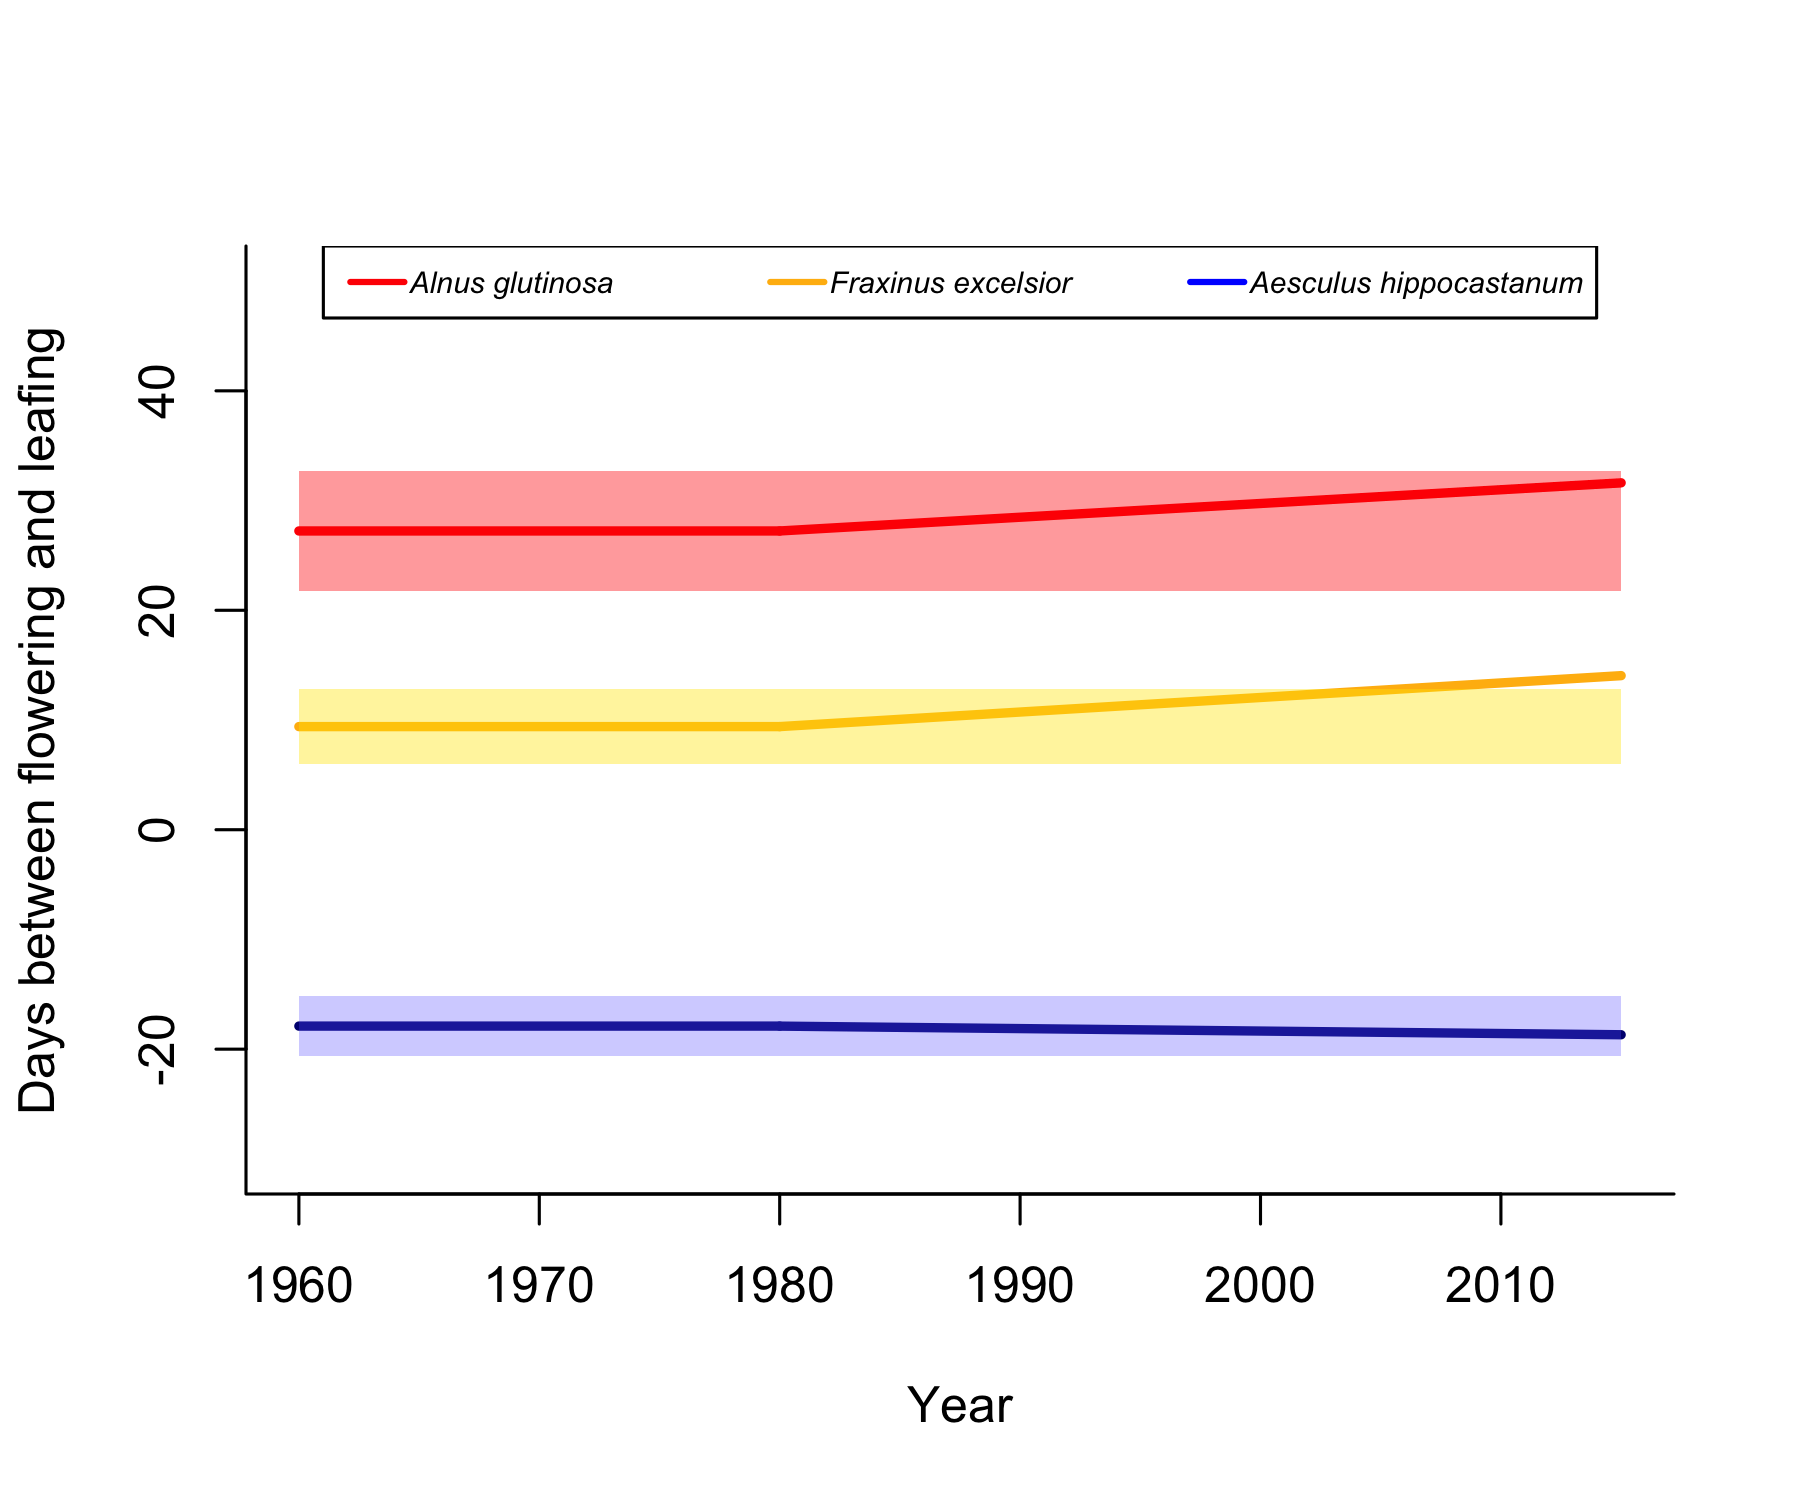
\includegraphics[width=\textwidth]{/PEP725/FLS_climate_change.png} 
    \caption{\textbf{FLSs across Europe for three tree species from 1960 to 2015 suggests climate change has generally increased the time between flowering and leafing}, but the direction and rate of change differs across species, which may exacerbate fitness differences within forest communities. To detect the effect of climate change on average FLS, we used models that allow for shifts in FLS after 1980. Lines represent the mean trend in FLS per species, and the highlighted regions indicate historic range of FLS variability (95\% credible intervals of the pre-1980 average) from the PEP725 database \citep{PEP725}.}
    \label{fig:climchage}
\end{figure}
\end{document}